\chapter{Conclusions and Outlook}
\label{cha:conclusions}

This work was concerned with axiomatizing all GCIs expressible in the description logic
$\ELbot$ that enjoy a certain minimal confidence in a given finite interpretation.  The
motivation for this research stemmed from the observation that the results from
Distel~\cite{Diss-Felix} on finding finite bases of finite interpretations are very
sensitive towards sporadic errors in the given interpretation, and thus may not perform
well on real-world data, which can be assumed to always contain errors.

The way errors affect the results obtained by Distel's results has been assessed in detail
in \Cref{sec:computing-bases-from}, where we have argued how \emph{linked data} can be
seen as a variant of finite interpretations, and where we have computed finite bases of a
finite interpretation $\Idbpedia$ that has been obtained from the DBpedia data set by
restriction to the \textsf{child} role.  Computing finite bases of the interpretation
$\Idbpedia$ turned out to be not very insightful, mostly because the concept names
contained in $\Idbpedia$ consisted mostly of job descriptions, and it cannot be expected
that the job of a parent affects the jobs of their children, or vice versa, in a way
expressible as a GCI.  Furthermore, the interpretation $\Idbpedia$ turned out to be
erroneous to the extent that it contained things that are usually not associated with the
\textsf{child} role, like places, books or bands.

Despite the deficits of $\Idbpedia$, we have argued that one still can expect certain GCIs
to be valid in $\Idbpedia$, most notably
\begin{equation*}
  \exists \mathsf{child}. \top \sqsubseteq \mathsf{Person}.
\end{equation*}
However, this GCI turned out to be not valid in $\Idbpedia$.  The reason for this was that
among the 2551 elements to which this GCI is applicable in $\Idbpedia$, 4 of them were
erroneously not an instance of \textsf{Person}.  In other words, the GCI $\exists
\mathsf{child}. \top \sqsubseteq \mathsf{Person}$ will not be collected by Distel's
approach because it is erroneously invalidated by a comparably small number of
counterexamples.

This observation motivated us to extend the results on axiomatizing valid GCIs into the
direction of axiomatizing GCIs with \emph{high confidence} in the given data.  This
extension has been discussed in \Cref{sec:confident-gcis}, where we had adapted results
obtain by Luxenburger~\cite{diss:Luxenburger} on \emph{partial implications} in finite
contexts to the setting of GCIs in finite interpretations $\mathcal{I}$.  From this
adaption we have obtained finite confident bases of finite interpretations
(\Cref{thm:conf-base}, \Cref{thm:luxenbuger-base-for-gcis}), and a way to compute finite
confident bases of GCIs from finite confident bases of implications
(\Cref{thm:confident-bases-of-GCIs-from-confident-bases-of-implications}).  We have also
seen how we can make use of the canonical base of the induced context $\con
K_{\mathcal{I}}$ of $\mathcal{I}$ to complete bases of $\Th_{c}(\mathcal{I}) \setminus
\Th(\mathcal{I})$ to confident bases of $\Th_{c}(\mathcal{I})$.  Finally, we have
generalized in \Cref{sec:unrav-elgfpb-bases} results of Distel to obtain finite confident
$\ELbot$ bases from finite confident $\ELgfpbot$ bases, using the technique of
\emph{unravelling} $\ELgfpbot$ concept descriptions.

The results we had obtained about computing finite confident bases of $\mathcal{I}$ were
then in turn applied to our example interpretation $\Idbpedia$, to examine how the
approach of computing finite confident bases performs on this data set.  As expected, we
could recover the GCIs $\exists \mathsf{child}. \top \sqsubseteq \mathsf{Person}$, as well
as another GCI.  In particular, we have observed that for relatively large values of the
confidence threshold $c$, the number of additional GCIs to be examined by the expert is
relatively small.  Thus, one could argue that the approach of considering GCIs with high
confidence does not add too much overhead for practical applications, but promises to
deliver more robust results.

However, the approach of considering GCIs with high confidence is still a heuristic
approach, and the GCIs thus obtained need to be validated by an external source of
information, like a human expert.  Indeed, the same is true for valid GCIs of the input
interpretation $\mathcal{I}$, as it may be the case that $\mathcal{I}$ misses some crucial
counterexamples for the domain of interest.  For this purpose, Distel developed
\emph{model exploration} to interactively consult an expert during the computation of a
finite base of $\mathcal{I}$ to provide missing counterexamples as needed.  We have argued
that providing such an exploration algorithm for the computation of finite confident bases
may also be helpful for practical applications.

To this end, we have first discussed in \Cref{cha:expl-conf} an approach to obtain an
exploration algorithm for \emph{implications with high confidence} in some given formal
context $\con K$, called \emph{exploration by confidence}.  For this, we have introduced
in \Cref{sec:an-abstract-view} an abstraction of the classical attribute exploration
algorithm as an algorithm to explore the set $\Th(\con K)$ of implications.  Then in
\Cref{sec:expl-conf-1}, we have argued how this abstraction can be transferred to the set
$\Th_{c}(\con K)$, automatically yielding an algorithm that explores the set $\Th_{c}(\con
K)$.  This algorithm, which indeed computes the canonical base of $\Th_{c}(\con K) \cap
\Th(p)$ with respect to some given expert $p$, has the practical disadvantage that it
requires the computation of closures under $\Th_{c}(\con K)$, which may not be feasible in
certain applications.  To remedy this, we have introduced in \Cref{sec:poss-fast-expl} an
exploration algorithm that avoids this computation, but does not necessarily compute the
canonical base of $\Th_{c}(\con K) \cap \Th(p)$ anymore.

The purpose of the then following \Cref{cha:model-expl-conf} was to extend the algorithm
for exploration by confidence to provide an algorithm for \emph{model exploration by
  confidence}.  Such an algorithm was obtained in \Cref{sec:expl-conf-gcis-1}.  As a
byproduct of the argumentation used, we also obtained more practical algorithms for
computing confident bases of formal contexts (\Cref{sec:grow-sets-attr-1}) and of finite
interpretations (\Cref{sec:expl-conf-gcis}).  Those algorithms compute the set
$M_{\mathcal{I}}$ incrementally, and not completely as a first step in the run, thus
avoiding this delay when computing implications and GCIs, respectively.

The work presented so far is not completed, and a lot remains to be done to turn the
results of this thesis into practically relevant techniques.  As a first step one could
extent the results of this thesis to also incorporate the notion of \emph{support} of
GCIs, an idea which is again borrowed from standard data mining
approaches~\cite{arules:agrawal:association-rules}.  More precisely, one could define for
a GCI $C \sqsubseteq D$ its support $\supp_{\mathcal{I}}(C \sqsubseteq D)$ in
$\mathcal{I}$ to be
\begin{equation*}
  \supp_{\mathcal{I}}( C \sqsubseteq D ) := \frac{ \abs{(C \sqcap D)^{\mathcal{I}}} }{
    \abs{ \Delta^{\mathcal{I}} } }.
\end{equation*}
Then one can consider only those GCIs whose support is above a given threshold $s \in
[0,1]$.  The idea behind this approach is that if the support of $C \sqsubseteq D$ is not
high enough in $\mathcal{I}$, then this data set does not contain enough information about
this GCI to decide whether $C \sqsubseteq D$ is true in the domain of discourse or not.
In this case, the GCI $C \sqsubseteq D$ should be ignored.

An adaption of the results presented in this thesis to include the support measure should
not be very difficult, and indeed results from formal concept analysis could again be used
here~\cite{DBLP:conf/ki/StummeTBPL01,arules:Stumme:2002}.  However, one could also step
back and ask whether the notions of support and confidence are really suitable for our
description logic setting: it has been argued in~\cite{DBLP:conf/icdm/BorchmannD11} that
the support (and also the confidence) of a GCI as defined above may be counter-intuitive,
at least as measures of trustworthiness.  To see this, let us consider the example as
given in~\cite{DBLP:conf/icdm/BorchmannD11}, which consisted of an interpretation that
contained an element for the Louvre in Paris, all pieces of art that are kept there, and
an element to represent the city of Paris.  The complete example interpretation is
sketched in \Cref{fig:support-of-gcis-can-be-counter-intuitive}.

\begin{figure}[t]
  \centering
  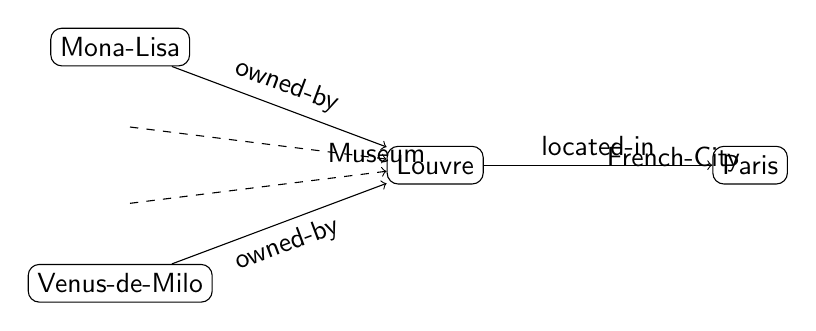
\begin{tikzpicture}[
    element/.style={rectangle,draw,rounded corners},
    every label/.style={anchor=north east},
    label distance=1ex,
    ]
    \node[element] (Mona-Lisa) at (0,0) {\textsf{Mona-Lisa}};
    \node (dummy-1) at (0,-1) {};
    \node (dummy-2) at (0,-2) {};
    \node[element] (Venus-de-Milo) at (0,-3) {\textsf{Venus-de-Milo}};
    \node[element,label=above:{\textsf{Museum}}] (Louvre) at (4,-1.5) {\textsf{Louvre}};
    \node[element,label={[label distance=0.7ex]above:{\textsf{French-City}}}] (Paris) at (8,-1.5) {\textsf{Paris}};
    \path {
      (Mona-Lisa) edge[->] node[midway,above,sloped] {\textsf{owned-by}} (Louvre)
      (Venus-de-Milo) edge[->] node[midway,below,sloped] {\textsf{owned-by}} (Louvre)
      (dummy-1) edge[->,dashed] (Louvre)
      (dummy-2) edge[->,dashed] (Louvre)
      (Louvre) edge[->] node [midway,above,sloped] {\textsf{located-in}} (Paris)
    };
  \end{tikzpicture}
  \caption{Support can be counter-intuitive}
  \label{fig:support-of-gcis-can-be-counter-intuitive}
\end{figure}

In this example interpretation, the GCI
\begin{equation*}
  \mathsf{Museum} \sqsubseteq \exists \text{\textsf{located-in}}. \text{\textsf{French-City}}
\end{equation*}
has very low support, because there is only one museum in the data set.  Therefore, one
could argue that this GCI is not very trustworthy.  Based on this, one could argue that
the GCI
\begin{equation*}
  \exists \text{\textsf{owned-by}}. \mathsf{Museum} \sqsubseteq \exists
  \text{\textsf{owned-by}}. \exists \text{\textsf{located-in}}. \text{\textsf{French-City}}
\end{equation*}
is not more trustworthy then the GCI before.  However, this GCI has very high support in
the example interpretation, because there are thousands of exhibits in the Louvre.
Therefore, the support measure would assign this GCI a very high trustworthiness, although
we would intuitively assign it a rather low one.  Finding a more intuitive approach to
measure trustworthiness and relevance of GCIs in a given data set remains an open problem.

But even if one accepts the way we have defined the confidence of an GCI, more work
remains to be done to make our approach more practically relevant.  For example, in
\Cref{thm:confident-bases-of-GCIs-from-confident-bases-of-implications} we have shown a
way how finite confident bases of finite interpretations can be obtained from bases of
implications with high confidence in the corresponding induced formal context.  What we
did not talk about was a way how to obtain such bases of implications with high
confidence.  To obtain these, it may prove fruitful to exploit the close connection of
formal concept analysis to data mining~\cite{arules:Zaki:1998}, and try to adapt known
algorithm from data mining for computing association rules to the setting of computing
bases of implications with high confidence.  In this way, one could hope to obtain much
faster implementations as those we have used for our
experiments~\cite{DBLP:conf/icdm/BorchmannD11}, and thus increase the practicability of
our approach to construct knowledge bases from large amounts of data.

Another usability issue concerns the way we have constructed our algorithm for model
exploration by confidence, as presented in \Cref{sec:expl-conf-gcis-1}.  There not only
the number of GCIs asked to the expert is quite high, probably much higher then in the
model exploration algorithm as proposed by Distel.  Moreover, if the GCIs are presented to
a human expert, extra care is needed.  More precisely, the GCIs
\begin{equation*}
  \bigsqcap P_{i} \sqsubseteq (\bigsqcap P_{i})^{\mathcal{I}_{\ell}\mathcal{I}_{\ell}}
\end{equation*}
we ask to the expert may contain proper $\ELgfpbot$ concept descriptions, and moreover the
size of the premises $P_{i}$ may be too large, both issues that may inhibit human
comprehension.

The former problem can be attacked by considering only those GCIs where the role-depth is
not larger than an a-priori chosen maximal role-depth $k \in \NN$.  More precisely, we can
define
\begin{equation*}
  \Th_{c}^{k}(\mathcal{I}) := \set{ (C \sqsubseteq D) \in \Th_{c}(\mathcal{I}) \mid d(C), d(D)
    \leq k },
\end{equation*}
and can then try to find small bases $\mathcal{B} \subseteq \Th_{c}^{k}(\mathcal{I})$ of
$\Th_{c}^{k}(\mathcal{I})$ (note that now $\Th_{c}^{k}(\mathcal{I})$ is finite, up to
equivalence).  In the case $c = 1$, where we only consider valid GCIs of $\mathcal{I}$,
all results obtained by Distel can be carried over, as sketched in~\cite{FCA-and-Logics}.
Indeed, limiting the role-depth of the concept descriptions involved eliminates the need
for the description logic \ELgfpbot, and thus simplifies the underlying theory
considerably.  Transferring these results to the setting of GCIs with high confidence
seems practically relevant.

To address the fact that $P_{i}$ may be too large to be understandable for human experts,
one could restrict oneself to only find bases of GCIs $C \sqsubseteq D$ where $C$ has at
most $\ell$ conjuncts, for some a-priori chosen value $\ell \in \NN$.  To solve the
problem of finding a small base for this set of GCIs (which is now finite), one could
first try to solve the simpler problem of finding a base of the set of valid implications
in a formal context $\con K = (G, M, I)$ where the premise has size of most $\ell$.  Note
that such a base would be
\begin{equation*}
  \set{ A \to A'' \mid A \subseteq M, \abs A \leq \ell }.
\end{equation*}
However, this base has size $\binom{\abs M}{\ell}$, which, although polynomial in $\abs
M$, may be too large for practical applications, and thus finding a smaller base is
necessary.  It would also be desirable to have an exploration algorithm that only asks
implications where the premise does not have more than $\ell$ elements.  As soon as those
problems are solved for the setting of implications, one should try to transfer them to
the setting of GCIs, probably again with an a-priori chosen role-depth for the concept
descriptions involved.

%%% Local Variables: 
%%% mode: latex
%%% TeX-master: "../main"
%%% End: 

%  LocalWords:  gcis thm luxenbuger conf expl attr de
